\subsection{Spectral Risk Measures}\label{subsec:spectral-risk-measures}
Variance and VaR cannot represent ... (give definitations)


Spectral Risk Measures takes a form of

\begin{equation}\label{eq:SRM}
	M_{w}(X)=- \int^1_{0} w(p)q_{s}(X)ds
	\end{equation}\\

\noindent where $w(p)$ is a weighting function defined over the full range of cumulative probabilities $p \in [0,1]$. $M_{w}$ is a coherent measure if and only if $w$ satisfies, \\

\begin{itemize}
			\item Nonnegativity: $w(p) \ge 0$.
			\item Increasingness: $w'(p) \ge 0$.
			\item Normalisation: $\int^1_{0}w(p)dp=1$.
\end{itemize}
The first property requires that the weights are non-negative, and the second property is intended to reflect user risk aversion. The third one requires that the probability-weighted weights should sum to 1. %However, a drawback with property 3 is that it does not rule out the ES from the set of SRMs. In this case, we use the following property with strong condition instead of the third one. \\
\begin{itemize}
			\item Strict increasingness: $w'(p) > 0$.
\end{itemize}

\noindent Note that VaR and ES are included to spectral risk measure as special cases. The weighting function of VaR is a Dirac delta function which gives the outcome an infinite weight and the others a zero weight. On the other hand, the ES gives all tail quantiles the same weight. Both of them are not a suitable weight function for capturing investor's risk attitudes. \\

By setting a 'well-behaved' risk-aversion function which indicates the weights will rise more rapidly when the degree of risk aversion is higher, we investigate the behaviors of the users in terms of different weight function when they determine the hedge ratios. \\

We also consider wildly used risk measure is Value at Risk, VaR, a quantile of the portfolio loss distribution ({\color{blue}\citealp{jurgen2011statistics}})
\begin{equation}\label{eq:VaR}
q_{\alpha}(X) = F^{-1}_{X}(\alpha), \quad \alpha \in (0,1).
\end{equation}\\
For any random variable $X$, and its cumulative distribution function $F_X$ is well defined.
Due to the inconsistency of coherent risk, the use of expected shortfall has been discussed intensively in finance and risk management ({\color{blue}\citealp{jurgen2011statistics}}). Expected shortfall (ES) measures are expressed as
\begin{equation}\label{eq:ES}
\mbox{ES}_{\alpha}(X) = \frac{1}{1-\alpha}\int^1_{\alpha}q_{s}(X)ds
\end{equation}\\

\subsection{Two Risk Spectra}
Recognising the importance of the weighting function, we investigate different utility functions, $U(x)$ defined over outcomes $x$. Consider the exponential utility and power utility, where the investor's coefficient of absolute risk aversion is $k(x)= -\frac{U''(x)}{U'(x)} $ and his relative risk-aversion is $\gamma(x)=-\frac{xU''(x)}{U'(x)}$. This allows us to transfer the utility function to a weighting function as in {\color{blue}\citet{dowd2008spectral}}.

\subsubsection{Exponential Spectral Risk Measure}
  The exponential SRM is specified by only one risk parameter $k$. To obtain the risk spectrum, we set $ w(p)= \lambda e^{-k(1-p)}$ and $\lambda = \frac{k}{1-e^{-k}}$. Then, the risk spectrum and its antiderivative are: 

\begin{equation}\label{eq:w}
 w(p)=\frac{ke^{-k(1-p)}}{1-e^{-k}},\quad \mbox{and} \quad  W(p)=-\frac{1-e^{-k(1-p)}}{1-e^{-k}}
\end{equation}\\

\noindent where $k \in (0, \infty),\quad p\in [0, 1]$. This function depends on only one $k$. Figure \ref{Fig1:EPSRM} shows the exponential risk spectrum and its antiderivative for $k=1$, and $2$. By substituting into (\ref{eq:SRM}), the exponential SRM is, 
\begin{equation}\label{eq:ESRM}
 M_{w}(X)= \int^1_{0} \frac{ke^{-k(1-p)}}{1-e^{-k}}F^{-1}(p)dp
\end{equation}

\subsubsection{Power Spectral Risk Measure}
The power weighting function only has one parameter, $\gamma$, which leads to $w(p)= \frac{\lambda (1-p)^{\gamma-1}}{1-\gamma}$ as $0<\gamma<1$. Then, by setting $\lambda =\gamma(1-\gamma)$, the risk spectrum and its antiderivative are, 
\begin{equation}\label{eq:wp}
 w(p)=\gamma(1-p)^{\gamma-1},\quad \mbox{and} \quad  W(p)=-(1-p)^{\gamma}
 \end{equation}\\
  Plugging the weighting function to (\ref{eq:SRM}), the power SRM is obtained,
 %By setting $\gamma= 0.5$ and $0.8$, power risk spectrum and its antiderivative are showed in Figure \ref{Fig2:PSRM}.  
 \begin{equation}\label{eq:PSRM}
 M_{w}(X)= \int^1_{0} \gamma(1-p)^{\gamma-1}F^{-1}(p)dp
\end{equation}
 For the case of $\gamma >1$, we have $w(p)= \frac{\lambda p^{\gamma-1}}{1-\gamma}$ with $\lambda =\gamma(1-\gamma)$. The risk spectrum is written as, 
\begin{equation}\label{eq:wp2}
 w(p)= \gamma p^{\gamma-1} 
\end{equation}\\
The Power SRM then becomes,
\begin{equation}\label{eq:PSRM2}
 M_{w}(X)= \int^1_{0} \gamma p^{\gamma-1}F^{-1}(p)dp
 \end{equation}\\

\begin{figure}
	\begin{center}
		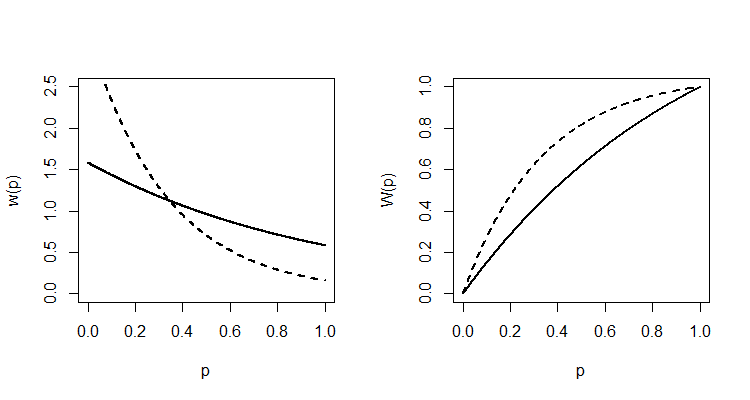
\includegraphics[scale = 0.7]{Figures/Fig1-1.png}\\
		%\vspace*{-10pt}\quantnet \href{https://github.com/mangrou/SRM/blob/master/SRM_QF/SRM_QF.m}{SRM\_QF} 
	\end{center}
	\caption{Exponential SRMs for $k=1$ (dashed) and $k=2$ (solid).}\label{Fig1:EPSRM}
\end{figure}

\begin{figure}
	\begin{center}
		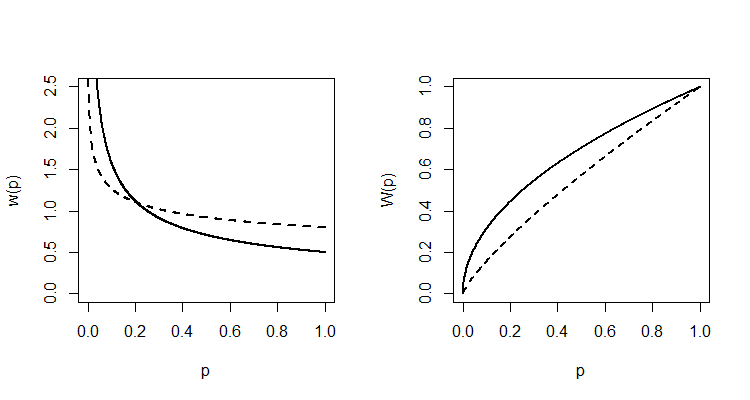
\includegraphics[scale = 0.7]{Figures/Fig2-1.png}\\
		%\vspace*{-10pt}\quantnet \href{https://github.com/mangrou/SRM/blob/master/SRM_QF/SRM_QF.m}{SRM\_QF} 
	\end{center}
	\caption{Power SRMs for $\gamma=0.5$ (solid) and $\gamma=0.8$ (dashed).}\label{Fig2:PSRM}
\end{figure}		
%%\subsubsection{Critical Parameter Region}
%%Following {\color{blue}\citet{brandtner2015decision}}, we try to restrict the relevant risk parameters $k$ and $\gamma$ which fall in the regions of strong risk aversion. The lower bound of risk parameter of exponential SRM, $k$, is set to $1.5937$ and $\gamma=$ is $0.5$ for power SRM.   {\color{blue}\citet{loomes1988different}} indicates the lower bound corresponds to a risk parameter of $k=5.7$ for exponential SRM measure, and of $\gamma= 0.115$ for power SRM for the binary lottery. {\color{blue}\citet{harrison2008risk}} indicate an average EU-function based on pooled utility function to yield $k=3.09$ and $\gamma= 0.37$. The parameters estimated from both literatures are lying in the problematic region of risk aversion. \\
%%
%%This paper discovers the hedge ratio is becoming less although he is ranked more risk averse that the risk aversion parameter of exponential SRM is beyond $1.5$. Moreover, if the risk aversion parameter of power SRM is beyond $0.8$, the hedge ratio becomes less. This empirical result is in line with the points of {\color{blue}\citet{brandtner2015decision}}.
%% 
%%Although those literatures provide the theoretical results of the threshold, this paper discovers the hedge ratio is becoming less although he is ranked more risk averse by minimizing exponential SRMs of the joint distribution of S\&P 500 spot and futures if risk aversion parameter beyond $9.8$. This result provides the reference of threshold to the risk aversion parameters in line with the points of {\color{blue}\citet{brandtner2015decision}}.
%
%
%
%
%\subsection{The Optimal Hedge Ratio}
%
%The optimal hedge ratio is defined as the ratio of the futures position to hedge the down size risk of selling one corresponding stock in the future ({\color{blue}\citealp{hull2016options}}). The hedge portfolio is: 
%
%\begin{equation*}
%        r_p=(r_s-\chi r_f)
%     \end{equation*}
%\noindent where $r_s$ and $r_f$ are denoted the return on the spot and the futures position, respectively. $\chi$ indicates the daily hedge ratio. Following {\color{blue}\citet{barbi2014copula}}, our purpose is to model the quantiles of $r_p$, where the dependence structure between $r_s$ and $r_f$ is modeled by a copula function, $C$. The $F^{-1}_{r_p}(\alpha)$ solves the following, 
%\begin{equation}\label{eq:QF}
%       1- \int^1_{0}  \frac{\partial }{\partial u} C\left[ u,1-F_{r_f} \left\lbrace \frac{F^{-1}_{r_p}(\alpha) - F^{-1}_{r_s}(u)}{\chi}\right\rbrace \right]  du=\alpha
%     \end{equation}
%
%\noindent The density of the copula is presented as, 
%\begin{equation}\label{eq:QFdensity}
% \int^1_{0} c\left[ u,1-F_{r_f} \left\lbrace \frac{F^{-1}_{r_p}(\alpha) - F^{-1}_{r_s}(u)}{\chi}\right\rbrace \right]  f_{r_p}\left\lbrace \frac{F^{-1}_{r_p}(\alpha) - F^{-1}_{r_s}(u)}{\chi}\right\rbrace du=f_{r_p}(\alpha)
%     \end{equation}
%\noindent where $f_{r_p}(x)=\frac{\partial }{\partial x}F_{r_p}(x)$. Equation (\ref{eq:QF}) defines the quantile function $F^{-1}_{r_p}(\alpha)$ implicitly. Thus, the optimal hedge ratio, $\chi$, is determined as, 
%
%\begin{equation}\label{eq:optimal}
%\hat{\chi}=\mbox{arg}\min_{\chi} M_{w}(r_p)	
%\end{equation}
%
%
%
%\section{Data}
%%\subsection{Financial Data}
%%
%%In this section, we illustrate how to proceed with the financial data. By assuming the S\&P 500 index and it corresponding futures index, S\&P 500 futures following the EGARCH(1,1),   
%%
%%\begin{equation*}
%%\begin{aligned}
%%&r_{i,t}=a_i+b_ir_{i,t-1}+\varepsilon_{i,t}.\\
%%&\varepsilon_{i,t} 
%%\mid \Omega_{t-1}= h_{i,t}z_{i,t}.\\
%%&z_{i,t}\sim iid\hspace{2mm}t_i.\\
%%&h^2_{i,t}=exp\{c_i+m_i\mbox{log}h^2_{i,t-1}+\beta_iz_{i,t-1}+\theta[\vert z_{i,t-1}\vert-\mathsf{E}(\vert z_{i,t-1}\vert)]\}.\\
%%&i=\{s,f\}.\\
%%\end{aligned}
%%\end{equation*}
%%
%%\noindent where $r_{i,t}$ are retuns and $\varepsilon_{i,t}$ are i.i.d vectors. By applying the different copulae, the parameters are computed from the EGARCH filtered data. 
%
%\subsection{Data Description}
%
%To demonstrate the application of copulae in optimal hedge ratio estimation, we collect daily data on six stock indices (FTSE 100, FTSE Mid 250, FTSE 350 and S\&P 500, S\&P Composite 1500 for the US market) and  two exchange rates (EURUSD and EURGBP). We use the FTSE 100 futures to hedge the spot position on all UK indices; the S\&P 500 to hedge the spot position on both US indices; currency futures on EURUSD and EURGBP to hedge the repective currency spot position. We draw daily data from Bloomberg and collect around 30 years of dat from January 1990 as possible. This is feasible for all UK spot and futures indices, for S\&P 500 spot and futures index. For the remaining series, we select the maximum spot and futures paired common time period, that is for currencies. Our dataset begins on 11 January 1999 (the euro was introduced as an accounting currency on 1 January 1999). For S\&P,  Composite 1500 it starts on 30 December 1994. 
%In total, we at most obtained 7898 pairs of daily observations for the index and index futures from 1999 to 2019 from Bloomberg. Futures prices are considered as a continuous series, by rolling over maturity on the first day of the delivery month. This is a common practice when dealing with futures data. ({\color{blue}\citealp{carchano2009rolling}}).
%Regardless of the maturities of futures price time series, the descriptive statistics are presented in Table \ref{TB1:Summary}. It reports the sample descriptive statistics. The summary statistics shows that they are skewed to the left except currency EURGBP, and the kurtosis coefficients are all greater than three except currency EURUSD which means heavy-tailed distribution. In particular, among stock indices, S\&P exhibits the highest kurtosis. The result is showing that the financial data is far from being Gaussian. \\
%Table \ref{TB2} shows the time-varying correlations between spot and futures series during the considered time period. On average, looking at the time period as a whole, correlations are generally high. UK and US stock indinces report an average correlation of about $97\%$, except for the FTSE 250 index, which correlates the less with the FTSE 100 futures ($78\%$). The average correlation diminishes as we pass to consider exchange rates ($94\%$ and $95\%$ for EURUSD and EURGBP, respectively).  However, the most important insight from Table \ref{TB2} is that correlations are not constant over time. Specifically, correlations are generally lower during the 199s and increase dramatically afterwards. 
%
%
%\begin{table}[ht]
%	\centering
%	\resizebox{\textwidth}{25mm}{
%	\begin{tabular}{lrrrrrrrr}
%		\hline
%		Spot & N & Average(\%) & SD(\%) & Minimum(\%) & Median(\%) & Maximum(\%) & Skewness & Kurtosis \\ 
%		\hline
%		S\&P 500 &  7898 & 0.0113 & 0.4890 & -5.5439 & 0.0113 & 4.7586 & -0.3968 & 12.2127 \\ 
%		S\&P 1500 &  6595 & 0.0121 & 0.5162 & -5.6081 & 0.0158 & 4.6787 & -0.4447 & 11.5959 \\ 
%		FTSE 100 &  7898 & 0.0047 & 0.4737 & -4.9998 & 0.0013 & 4.0756 & -0.2915 & 8.2525 \\ 
%		FTSE 250 &  7898 & 0.0099 & 0.4074 & -4.2649 & 0.0202 & 3.4912 & -0.5345 & 9.7249 \\ 
%		FTSE 350 &  7898 & 0.0054 & 0.4524 & -4.8701 & 0.0061 & 3.8882 & -0.3429 & 8.7289 \\ 
%		EURUSD &  7898 & -0.0006 & 0.2647 & -1.4687 & 0.0000 & 1.4986 & -0.0076 & 1.9539 \\ 
%		EURGBP &  7898 & 0.0008 & 0.2387 & -1.3604 & -0.0033 & 2.6109 & 0.2390 & 3.7460 \\ 
%		\hline
%		Futures &  &  & & & & & & \\ 
%		 \hline
%		S\&P 500 &  7898 & 0.0111 & 0.4972 & -4.7571 & 0.0157 & 5.7315 & -0.2701 & 12.6629 \\ 
%		FTSE 100 &  7898 & 0.0046 & 0.4929 & -4.3790 & 0.0000 & 4.1607 & -0.2581 & 6.7389 \\ 
%		FTSE 250 &  1647 & 0.0013 & 0.4288 & -4.0818 & 0.0149 & 3.2992 & -1.3365 & 18.3208 \\ 
%		EURUSD &  5712 & -0.0002 & 0.2589 & -1.3276 & 0.0000 & 1.4281 & -0.0282 & 1.6687 \\ 
%		EURGBP &  5543 & 0.0017 & 0.2174 & -1.5530 & 0.0000 & 2.6138 & 0.4844 & 7.2533 \\ 		
%		\hline\hline
%	\end{tabular}
%}
%\caption{{Descriptive Statistics for the sample of spot and futures returns}\\ Daily prices are taken from Bloomberg. Sample periods are from January 1990-December 2019 (UK indices, S\&P 500), while the start date is postponed to January 1995 for S\&P Composite 1500, January 1999 for currencies. }\label{TB1:Summary}
%\end{table}
%
%
%
% \begin{table}[h!]
%		\begin{center}
%			\resizebox{\textwidth}{25mm}{
%			\begin{tabular}{lrrrrrrrr}
%				\hline\hline
%				Spot & Futures & 1990-2019 & 1990-1994 & 1995-1999 & 2000-2004 & 2005-2009 & 2010-2014 & 2015-2019 \\
%				 \hline
%				S\&P 500 & S\&P 500 & 0.980& 0.964 & 0.961 & 0.972 & 0.982 & 0.980 & 0.980 \\ 
%				S\&P 1500 & S\&P  500 & 0.980 & - & 0.958 & 0.971 & 0.981 & 0.980 & 0.980 \\
%				FTSE 100 & FTSE 100 & 0.970 & 0.921 & 0.961 & 0.975 & 0.985 & 0.970 & 0.970 \\ 
%				%FTSE 100 & FTSE 250 & 0.780 & - & - & - & - & 0.780 & 0.780 \\ 
%				FTSE 250 & FTSE 100 & 0.780 & 0.751 & 0.647 & 0.694 & 0.854 & 0.880 & 0.780 \\ 
%				FTSE 250 & FTSE 250 & 0.980 & - & - & - & - & 0.970 & 0.980 \\ 
%				FTSE 350 & FTSE 100 & 0.960 & 0.917 & 0.957 & 0.974 & 0.984 & 0.970 & 0.960 \\ 
%				FTSE 350 & FTSE 250 & 0.830 & - & - & - & - & 0.830 & 0.830 \\ 
%				EURUSD & EURUSD & 0.940 & - & - & 0.947& 0.935 & 0.930 & 0.940 \\ 
%				EURGBP & EURGBP & 0.950 & - & - & 0.731 & 0.956 & 0.960 & 0.950\\   
%				\hline \hline
%			\end{tabular}
%		}
%		\end{center}
%		\caption{{Average correlations between spot and futures daily returns over time, and the overall average correlation over the considered time (1990-2014, except for the S\&P Composite 1500, currencies. )}\\
%                 SD stands for standard deviation}\label{TB2}
%	\end{table}	
%\begin{sidewaystable}[h]
%
%	\centering
%	\resizebox{\textwidth}{25mm}{
%	\begin{tabular}{llrrrrrrrrrrrrrrrr}
%		\hline\hline
%		&&k=10&&&&k=50&&&&k=100&&&&k=200\\
%		\hline
%		Spot & Futures & Gaussian & t & Clayton & Frank & Gaussian & t & Clayton & Frank & Gaussian & t & Clayton & Frank & Gaussian & t & Clayton & Frank \\ 
%		\hline
%	S\&P 500 & S\&P 500 & 0.912 & 0.912 & 0.930 & 0.912 & 0.912 & 0.850 & 0.912 & 0.904 & 0.912 & 0.912 & 0.912 & 0.912 & 0.896 & 0.896 & 0.896 & 0.945 \\ 
%	S\&P 1500 & S\&P  500 & 0.860 & 0.831 & 0.838 & 0.821 & 0.817 & 0.813 & 0.817 & 0.817 & 0.830 & 0.830 & 0.830 & 0.830 & 0.886 & 0.813 & 0.813 & 0.824 \\ 
%	FTSE 100 & FTSE 100 & 1.078 & 1.078 & 1.069 & 1.021 & 1.072 & 1.072 & 1.050 & 1.120 & 1.083 & 1.083 & 1.129 & 1.064 & 1.064 & 1.064 & 1.064 & 1.079 \\ 
%	FTSE 250 & FTSE 100 & 1.025 & 1.025 & 1.064 & 1.078 & 1.061 & 1.061 & 1.059 & 1.030 & 1.072 & 1.072 & 1.064 & 1.064 & 1.074 & 1.074 & 1.074 & 1.018 \\ 
%	FTSE 250 & FTSE 250 & 0.844 & 0.844 & 0.844 & 0.721 & 1.057 & 1.057 & 1.057 & 0.844 & 1.127 & 1.127 & 1.127 & 0.897 & 0.844 & 0.844 & 0.844 & 0.844 \\ 
%	FTSE 350 & FTSE 100 & 1.064 & 1.064 & 1.074 & 1.064 & 1.021 & 1.021 & 1.038 & 1.022 & 1.014 & 1.014 & 1.030 & 1.029 & 1.067 & 1.067 & 1.073 & 1.071 \\ 
%	FTSE 350 & FTSE 250 & 1.127 & 1.127 & 0.844 & 0.844 & 0.844 & 0.844 & 0.844 & 0.844 & 0.844 & 0.844 & 0.844 & 0.844 & 0.844 & 0.844 & 1.054 & 0.844 \\ 
%	EURUSD & EURUSD & 0.884 & 0.884 & 1.016 & 1.049 & 0.990 & 0.990 & 1.049 & 1.012 & 1.007 & 1.007 & 1.024 & 1.094 & 1.073 & 1.073 & 1.119 & 1.073 \\ 
%	EURGBP & EURGBP & 0.875 & 0.875 & 0.946 & 0.821 & 0.868 & 0.868 & 0.839 & 0.839 & 0.868 & 0.868 & 0.899 & 0.899 & 0.851 & 0.851 & 0.878 & 0.878 \\ 
%	\hline\hline
%	\end{tabular}
%
%}
%\caption{{ Risk measures ERM whose risk spectrum is computed as $\frac{ke^{-k(1-p)}}{1-e^{-k}}$ for different values of the risk-aversion parameter, $k=10,50,100, 200$. Optimal hedge ratios are numerically computed by employing Gaussian, t, Clayton, and Frank coupla within the interval $\chi \in [0,2]$. }}\label{TB3}
%\end{sidewaystable}
%
%\begin{sidewaystable}[h]
%
%	\centering
%		\resizebox{\textwidth}{25mm}{
%	\begin{tabular}{llrrrrrrrrrrrrrrrr}
%		\hline\hline
%		&&k=10&&&&k=50&&&&k=100&&&&k=200\\
%		\hline
%		Spot & Futures & Gaussian & t & Clayton & Frank & Gaussian & t & Clayton & Frank & Gaussian & t & Clayton & Frank & Gaussian & t & Clayton & Frank \\ 
%		\hline
%S\&P 500 & S\&P 500 & 33.814 & 38.798 & 28.364 & 31.132 & 54.568 & 59.986 & 55.437 & 60.220 & 74.920 & 70.001 & 89.273 & 76.559 & 80.241 & 91.317 & 71.773 & 88.429 \\ 
%S\&P 1500 & S\&P  500 & 22.871 & 32.999 & 28.563 & 17.658 & 69.911 & 61.774 & 51.861 & 77.193 & 85.481 & 78.789 & 87.087 & 86.246 & 93.169 & 91.844 & 86.655 & 89.643 \\ 
%FTSE 100 & FTSE 100 & 33.584 & 25.058 & 16.770 & 28.116 & 61.403 & 64.668 & 74.499 & 55.733 & 71.349 & 50.023 & 66.138 & 79.556 & 68.978 & 95.682 & 84.758 & 74.778 \\ 
%FTSE 250 & FTSE 100 & 30.084 & 34.479 & 19.898 & 31.599 & 61.803 & 51.637 & 83.963 & 58.590 & 67.908 & 81.406 & 68.085 & 71.678 & 87.258 & 95.253 & 94.100 & 83.709 \\ 
%FTSE 250 & FTSE 250 & 30.321 & 30.895 & 33.360 & 14.903 & 74.442 & 66.565 & 68.999 & 68.434 & 68.089 & 84.845 & 63.363 & 78.544 & 46.787 & 71.227 & 82.487 & 68.748 \\ 
%FTSE 350 & FTSE 100 & 21.101 & 38.074 & 17.215 & 30.615 & 66.373 & 76.581 & 50.438 & 80.746 & 85.867 & 87.246 & 84.649 & 70.232 & 84.797 & 94.362 & 81.758 & 89.652 \\ 
%FTSE 350 & FTSE 250 & 17.537 & 18.910 & 24.017 & 28.306 & 71.080 & 70.428 & 55.334 & 64.546 & 70.772 & 82.099 & 75.778 & 83.707 & 79.084 & 75.809 & 93.772 & 86.089 \\ 
%EURUSD & EURUSD & 31.562 & 33.946 & 33.480 & 36.584 & 65.384 & 73.455 & 69.224 & 71.995 & 81.246 & 72.280 & 73.939 & 84.373 & 86.337 & 88.065 & 90.596 & 89.791 \\ 
%EURGBP & EURGBP & 26.448 & 22.900 & 15.944 & 12.199 & 63.195 & 63.663 & 57.152 & 70.825 & 83.902 & 80.827 & 83.990 & 82.230 & 82.992 & 87.950 & 83.966 & 84.220 \\ 
%\hline\hline
%	\end{tabular}
%}
%\caption{{ Risk measures ERM whose risk spectrum is computed as $\frac{ke^{-k(1-p)}}{1-e^{-k}}$ for different values of the risk-aversion parameter, $k=10,50,100, 200$. Hedging effectiveness is measured as the percentage reduction of portfolio risk attributable to hedging, that is 1 minus the ratio between the risk of the optimally hedged portfolio and the risk of the unhedged portfolio.}}\label{TB4}
%
%\end{sidewaystable}
%
%
%
%\begin{sidewaystable}[h]
%	
%	\centering
%	\resizebox{\textwidth}{25mm}{
%		\begin{tabular}{llrrrrrrrrrrrrrrrr}
%			\hline\hline
%			&&k=10&&&&k=50&&&&k=100&&&&k=200\\
%			\hline
%			Spot & Futures & Gaussian & t & Clayton & Frank & Gaussian & t & Clayton & Frank & Gaussian & t & Clayton & Frank & Gaussian & t & Clayton & Frank \\ 
%			\hline
%			S\&P 500 & S\&P 500 & 1.699 & 1.699 & 1.699 & 1.699 & 1.699 & 1.699 & 1.699 & 1.815 & 1.749 & 1.749 & 1.749 & 1.749 & 1.247 & 1.247 & 1.247 & 1.602 \\ 
%			S\&P 1500 & S\&P  500 & 1.506 & 1.506 & 1.506 & 1.488 & 1.502 & 1.502 & 1.502 & 1.502 & 1.564 & 1.564 & 1.564 & 1.656 & 1.456 & 1.456 & 1.456 & 1.293 \\ 
%			FTSE 100 & FTSE 100 & 1.533 & 1.533 & 1.533 & 1.533 & 1.533 & 1.533 & 1.533 & 1.533 & 1.162 & 1.162 & 1.162 & 1.533 & 1.575 & 1.544 & 1.575 & 1.533 \\ 
%			FTSE 250 & FTSE 100 & 1.533 & 1.533 & 1.533 & 1.533 & 1.533 & 1.533 & 1.533 & 1.533 & 1.533 & 1.533 & 1.178 & 1.533 & 0.718 & 1.544 & 1.575 & 1.533 \\ 
%			FTSE 350 & FTSE 100 & 1.533 & 1.463 & 1.533 & 1.533 & 1.355 & 1.463 & 1.533 & 1.533 & 0.842 & 0.842 & 0.842 & 1.533 & 1.575 & 1.544 & 1.575 & 1.533 \\ 
%			EURUSD & EURUSD & 1.792 & 1.792 & 1.842 & 1.792 & 1.792 & 1.792 & 1.792 & 1.792 & 1.660 & 1.124 & 1.660 & 1.660 & 1.792 & 1.792 & 1.792 & 1.792 \\ 
%			EURGBP & EURGBP & 1.803 & 1.803 & 1.803 & 1.803 & 1.803 & 1.803 & 1.803 & 1.803 & 1.803 & 1.803 & 1.803 & 1.803 & 1.803 & 1.803 & 1.803 & 1.803 \\ 
%			\hline\hline
%		\end{tabular}
%		
%	}
%	\caption{{ Risk measures ERM whose risk spectrum is computed as $\frac{ke^{-k(1-p)}}{1-e^{-k}}$ for different values of the risk-aversion parameter, $k=10,50,100, 200$. Optimal hedge ratios are numerically computed by employing Gaussian, t, Clayton, and Frank coupla within the interval $\chi \in [0,2]$ during 2007-2008. }}\label{TB5}
%\end{sidewaystable}
%
%\begin{sidewaystable}[h]
%	
%	\centering
%	\resizebox{\textwidth}{25mm}{
%		\begin{tabular}{llrrrrrrrrrrrrrrrr}
%			\hline\hline
%			&&k=10&&&&k=50&&&&k=100&&&&k=200\\
%			\hline
%			Spot & Futures & Gaussian & t & Clayton & Frank & Gaussian & t & Clayton & Frank & Gaussian & t & Clayton & Frank & Gaussian & t & Clayton & Frank \\ 
%			\hline
%			S\&P 500 & S\&P 500 & 36.993 & 27.857 & 18.408 & 20.172 & 69.464 & 31.418 & 44.283 & 68.940 & 89.510 & 77.586 & 69.902 & 80.468 & 80.919 & 95.673 & 82.801 & 93.582 \\ 
%			S\&P 1500 & S\&P  500 & 28.313 & 10.025 & 10.692 & 22.406 & 66.619 & 68.904 & 65.922 & 63.782 & 86.180 & 81.198 & 90.368 & 77.818 & 91.574 & 77.003 & 74.282 & 75.102 \\ 
%			FTSE 100 & FTSE 100 & 29.104 & 23.124 & 21.901 & 33.026 & 87.537 & 67.005 & 57.399 & 74.268 & 63.581 & 79.343 & 90.640 & 78.584 & 90.075 & 79.884 & 93.625 & 88.849 \\ 
%			FTSE 250 & FTSE 100 & 29.126 & 25.574 & 30.508 & 16.006 & 55.524 & 70.432 & 61.857 & 68.255 & 74.676 & 90.072 & 77.292 & 66.480 & 84.160 & 86.309 & 76.883 & 83.903 \\ 
%			FTSE 350 & FTSE 100 & 38.841 & 29.541 & 19.498 & 30.711 & 77.274 & 69.313 & 79.618 & 77.289 & 61.829 & 74.697 & 64.267 & 83.610 & 86.917 & 87.438 & 85.821 & 86.363 \\ 
%			EURUSD & EURUSD & 15.752 & 32.076 & 25.045 & 17.088 & 60.903 & 67.348 & 50.829 & 61.143 & 82.536 & 83.228 & 44.783 & 67.427 & 79.179 & 75.343 & 91.407 & 93.630 \\ 
%			EURGBP & EURGBP & 14.636 & 21.775 & 13.228 & 19.811 & 79.253 & 75.383 & 73.598 & 77.228 & 75.944 & 71.064 & 80.766 & 67.496 & 82.077 & 91.392 & 79.982 & 90.076 \\ 
%			\hline\hline
%		
%		\end{tabular}
%	}
%	\caption{{ Risk measures ERM whose risk spectrum is computed as $\frac{ke^{-k(1-p)}}{1-e^{-k}}$ for different values of the risk-aversion parameter, $k=10,50,100, 200$. Hedging effectiveness is measured as the percentage reduction of portfolio risk attributable to hedging, that is 1 minus the ratio between the risk of the optimally hedged portfolio and the risk of the unhedged portfolio during 2007-2008.}}\label{TB6}
%	
%\end{sidewaystable}
%
%
%\section{Empirical Result}
%
%The hedged portfolio composed by a long spot position and an opposite futures position. We choose 4 different kinds of copulae, Gaussian, $t$, Clayton and Frank to capture the dependence structure between the spot and its corresponding futures. 
%%Within the Archimedean family, Clayton copula exhibits mass lower tail and less on the upper. Gumbel copula shows strong linkage on the upper, but also shows more variability and more mass in the lower tail.\\ 
%SRM composed of quantile function and weighting function as presented in eq.(\ref{eq:SRM}). By applying different copulas, it shows the quantile function derived from eq.(\ref{eq:QF}).  By setting different hedge ratios $\chi = 0.4, 0.5, 0.6$, Fig. \ref{Fig3:QF1} shows the quantile function by plugging 4 different copulae functions. By employing the value of $k$ from $1$ to $20$, the exponential SRM can be estimated. As can be seen in Figure 4, the more risk averse $k$ becomes, the higher spectral risk it measures. However, the solid lines ($\chi = 0.4$) by conducting 4 different copulae will shift inward which indicates that spectral risk measurement goes lower when hedge ratio is high.\\
%%On the other hand, power SRM is also estimated by restricting $0<\gamma < 1$. Looking at the relationship between $\gamma$ and power SRM in Fig. \ref{Fig5:PSRM_r}, the power SRM declines while $\gamma$ is increasing in $(0,1)$. Although the dashed line ($\chi = 0.4$) is below the solid line ($\chi = 0.3$), in this case, the risk measurement subsequently falls as the user becomes more risk aversion that is odd. On the other hand, if $\gamma >1$, the power SRM with respect to $\gamma$ is increasing in Fig \ref{Fig6:PSRM2_r}. \\
%
%Having a close look at the relationship between SRMs and hedge ratio in Fig. \ref{Fig5:ESRM_HR}, we set $k=5$ (solid) and $10$ (dashed), and estimate the exponential SRM by employing $\chi$ from $0$ to $1$. Fig. \ref{Fig5:ESRM_HR} shows that the minimum exponential SRM of portfolio is reached by selecting the optimal hedge ratio. It is reasonable that the dashed line represents more risk aversion ($k=10$) is lying above the solid line ($k=5$), the less risk aversion, as hedge ration is larger than $0.2$. This is a proper property to describe the investor behaviour.   \\
%
%The optimal hedge ratios are obtained by (\ref{eq:optimal}) based on the estimated joint probability distribution of index and futures conducted by different copulae. Table \ref{TB3}  shows that the optimal hedge ratios are derived by minimizing the exponential SRM in terms of different degrees of risk aversion coefficient, $k= 10, 50, 100, 200$ by employing different copulae. For each portfolio we compute the optimal hedge ratios using rolloing windows of length 260 trading days. The copula dependence parameter is re-estimated every 260 observation. 
%This procedure leads to 30 windows for S\&P500, and FTSE 100, FTSE250, and FTSE 100 ( this three UK indices with FTSE 100 futures), 20 windows for 2 exchange rates, and S\&P1500, and 6 windows for FTSE 250 and FTSE 350 with FTSE 250 futures. Table \ref{TB3} shows the average optimal hedge ratios of each portfolio.\\
%
%The hedging effectiveness of copula-based model applied to ESRM is presented inTable \ref{TB4}. We use $k= 10, 50, 100, 200$ as the ESRM absolute risk aversion parameter. There is a positive relationship between the absolute risk aversion and the hedging effectiveness. This is not surprising. Intuitively, as k increases, the more emphasis is attributed to negative events, and it is expected that hedgeing effectiveness is increased. \\
%
%Having a look at crisis period, the optimal hedge ratios are estimated during 2007-2008. The results are in Table \ref{TB5}. Compared with Table \ref{TB3}, the optimal hedge ratios in crisis period is generally higher than the ones in overall periods. 
%
%
%\begin{figure}
%\begin{center}
%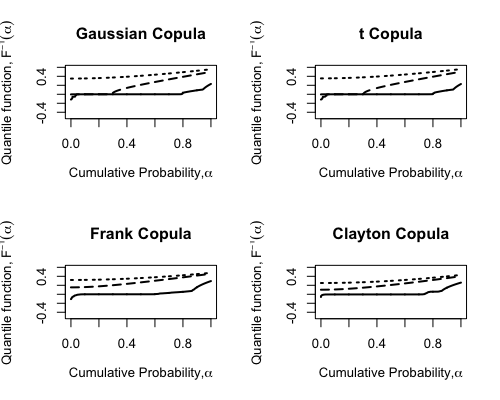
\includegraphics[scale = 0.75]{Figures/Fig3_20200726.png}\\
%%\vspace*{-10pt}\quantnet \href{https://github.com/mangrou/SRM/blob/master/SRM_QF/SRM_QF.m}{SRM\_QF} 
%\end{center}
%\caption{Setting $\chi = 0.4$ (solid), $0.5$ (dashed), and $0.6$ (dotted), quantile functions are estimated from (\ref{eq:QF}) by plugging Gaussian, $t$, Frank and Clayton copulae, respectively.}\label{Fig3:QF1}
%\end{figure}	
%
%
%%\begin{figure}
%%\begin{center}
%%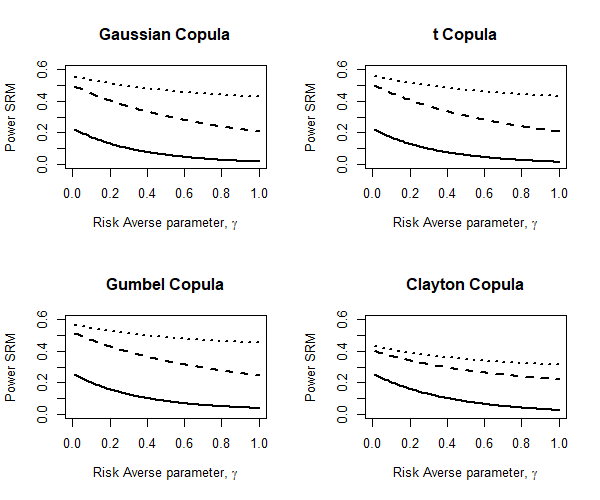
\includegraphics[scale = 0.8]{Figures/Fig5_20181001.png}\\
%%%\vspace*{-10pt}
%%%\quantnet \href{https://github.com/mangrou/SRM/tree/master/SRM}{ESRM} 
%%\end{center}
%%\caption{By setting setting $\chi = 0.4$ (solid), $0.5$ (dashed), and $0.6$ (dotted), power SRM is estimated from eq. (\ref{eq:PSRM}) as $0<\gamma<1$ by conducting Gaussian, $t$, Gumbel, Clayton copulae.}\label{Fig5:PSRM_r}
%%\end{figure}
%
%\begin{figure}
%\begin{center}
%	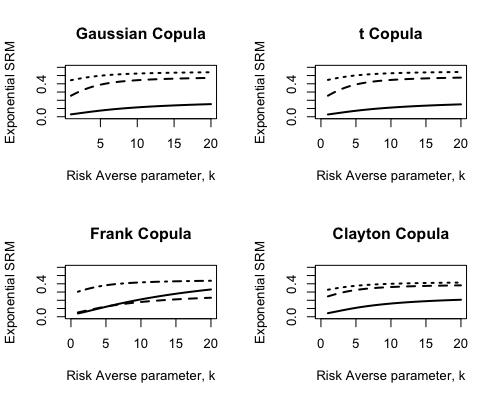
\includegraphics[scale = 0.75]{Figures/Fig5_20200726.png}\\
%	%\vspace*{-10pt}
%	%\quantnet \href{https://github.com/mangrou/SRM/tree/master/SRM}{ESRM} 
%\end{center}
% \caption{By setting $\chi = 0.4$ (solid), $0.5$ (dashed), and $0.6$ (dotted), exponential SRM is estimated from eq. (\ref{eq:ESRM}) by conducting Gaussian, $t$, Frank and Clayton copulae.}\label{Fig4}
%\end{figure}
%
%\begin{figure}
%\begin{center}
%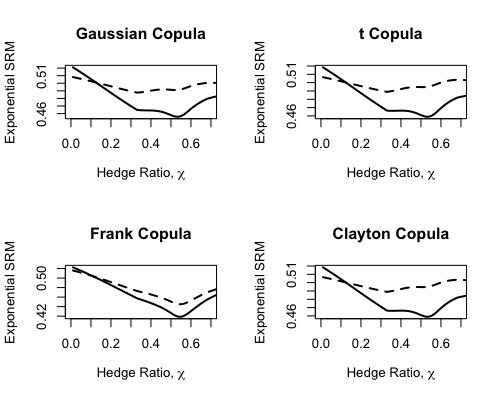
\includegraphics[scale = 0.8]{Figures/Fig6_20200726.png}\\
%%\vspace*{-10pt}
%%\quantnet \href{https://github.com/mangrou/SRM/tree/master/SRM}{ESRM} 
%\end{center}
%\caption{By setting $k = 5$ (solid) and $10$ (dashed), exponential SRM are estimated from (\ref{eq:ESRM}) by conducting Gaussian, $t$, Frank, Clayton copulae.}\label{Fig5:ESRM_HR}
%\end{figure}
%
% 
%   
%%\begin{figure}
%%\begin{center}
%%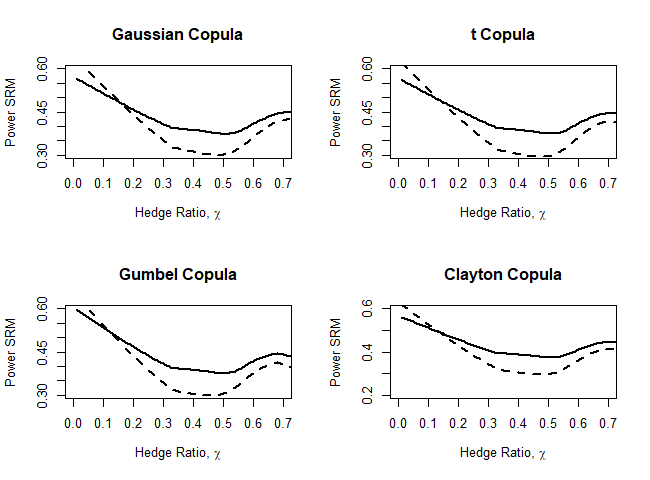
\includegraphics[scale = 0.8]{Figures/Fig8_20181002.png}\\
%%%\vspace*{-10pt}
%%%\quantnet \href{https://github.com/mangrou/SRM/tree/master/SRM}{ESRM} 
%%\end{center}
%%\caption{By setting $\gamma = 0.5$ (solid), $0.8$ (dashed), Power SRM is estimated from (\ref{eq:PSRM}) as $0<\gamma<1$ by conducting Gaussian, $t$, Gumbel, Clayton copulae}\label{Fig8:PSRM_HR}
%%\end{figure}
%
%
%%\begin{figure}
%%	\begin{center}
%%		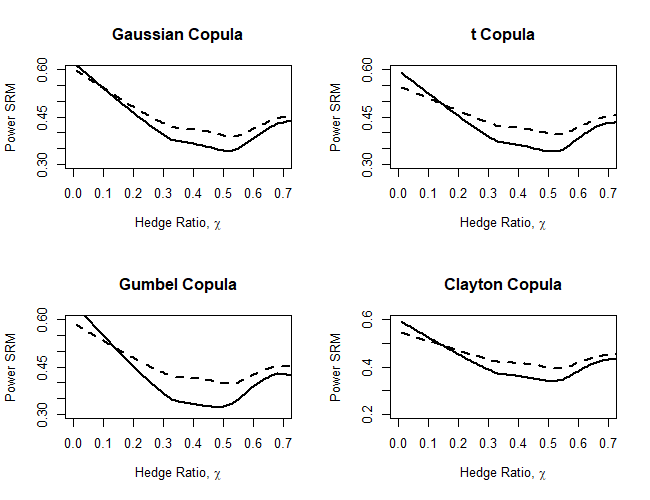
\includegraphics[scale = 0.8]{Figures/Fig9_20181002.png}\\
%%		%\vspace*{-10pt}
%%		%\quantnet \href{https://github.com/mangrou/SRM/tree/master/SRM}{ESRM} 
%%	\end{center}
%%	\caption{By setting $\gamma = 1.5$ (solid), $2$ (dashed), Power SRM is estimated from eq. (\ref{eq:PSRM2}) as $\gamma >1$ by conducting Gaussian, $t$, Gumbel, Clayton copulae}\label{Fig9:PSRM_HR}
%%\end{figure}
%
%
%
%
%
%
%
%\section{Conclusion}
%
%%We employ {\color{blue}\citet{barbi2014copula}} to illustrate the quantiles of the hedged portfolio in terms of a copula function. This method allows to estimate the hedged portfolio cumulative distribution function and separately choose the risk-minimizing hedge ratio. \\
%%
%%The general lesson of SRM is that users must be careful to ensure that utility functions should fit the features of the particular problems. By empirically investigating the relationship between the risk-aversion and the optimal hedge ratio, the exponential and power weighting function given $\gamma >1$ are more reasonable to illustrate the investors' risk attitude. The higher risk-averse it becomes the larger spectral risk it measures. 
%%%On the other hand, in our model, the optimal hedge ratio is much less successful to describe the investors behaviors. 
%%The higher risk measurement implies more willingness to pay for hedge ratio. As a consequence, these SRMs exhibit counter-intuitive results with respect to risk aversion. Spectral risk measurement is composed of the utility function of investor and the quantile function of assets. These two function will affect the investors behaviour. %To sum up, There is no conclusive summary about the optimal hedge ratio with respect to risk aversion parameter. \\ 
%%
%%This paper presents an approach to hedging with futures contracts which takes into two considerations that attract seldom adequate attention: Firstly, the quantiles of the hedged portfolio in terms of a copula function. Secondly, this paper implements different SRM by using empirical data to investigate which is reasonable to present the investors risk attitudes. Nonetheless, the results provide some sense of properties of different SRM applying to determine the optimal hedge ratio. \\
%
%%%%%%%%%%%%%%%%%%%%%%%%%%%%%%%%%%%%%%%%%%%%%%%%%%%%%%%%%%%%%%%%%%%%%%%%%
%

